\documentclass[tikz,border=8pt]{standalone}
\usetikzlibrary{arrows.meta,shapes.geometric}
\definecolor{bg}{HTML}{FBFBFB}
\definecolor{untrusted}{HTML}{FDECEC}
\definecolor{untrustededge}{HTML}{C0392B}
\definecolor{dmz}{HTML}{FFF6DD}
\definecolor{dmzedge}{HTML}{C98A1B}
\definecolor{mesh}{HTML}{E7F3EA}
\definecolor{meshedge}{HTML}{2E7D4F}
\definecolor{idpzone}{HTML}{EAF0FB}
\definecolor{idpedge}{HTML}{2A6F97}
\definecolor{idtok}{HTML}{7B5EA7}
\definecolor{acctok}{HTML}{2A6F97}
\definecolor{svctok}{HTML}{2E7D4F}
\definecolor{ink}{HTML}{233044}
\definecolor{node}{HTML}{FFFFFF}
\begin{document}
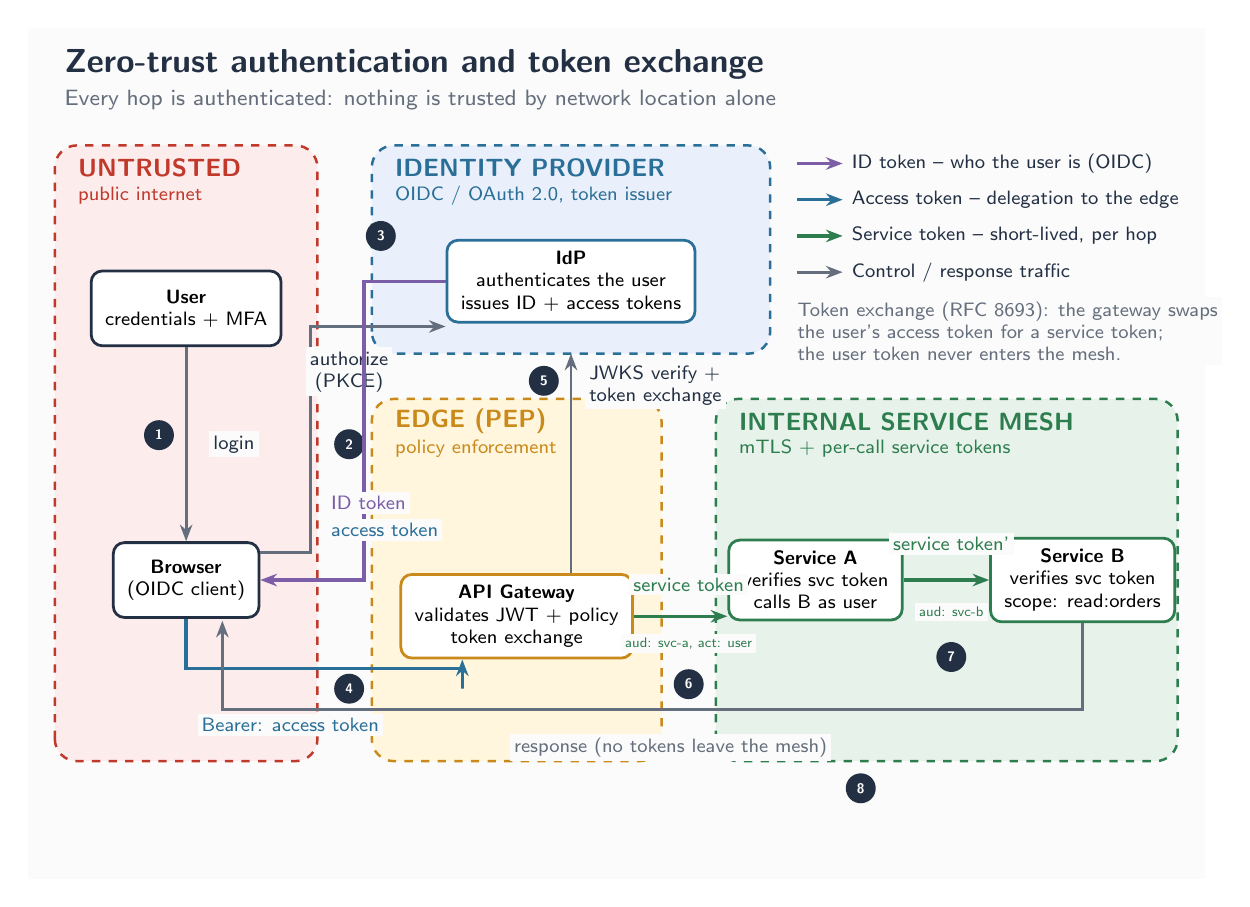
\begin{tikzpicture}[x=1.15cm,y=1.15cm,font=\sffamily\footnotesize,
  actor/.style={draw=ink,fill=node,line width=1pt,rounded corners=4pt,align=center,inner xsep=5pt,inner ysep=4pt,minimum height=0.95cm,font=\sffamily\scriptsize},
  idarrow/.style={-{Stealth[length=6pt]},line width=1.2pt,idtok},
  accarrow/.style={-{Stealth[length=6pt]},line width=1.2pt,acctok},
  svcarrow/.style={-{Stealth[length=6pt]},line width=1.2pt,svctok},
  plain/.style={-{Stealth[length=6pt]},line width=1pt,ink!70!white},
  stepn/.style={circle,fill=ink,text=white,font=\sffamily\bfseries\tiny,inner sep=1.5pt,minimum size=0.38cm},
  lbl/.style={font=\sffamily\scriptsize,fill=bg,inner sep=1.5pt,align=center},
  zone/.style={font=\sffamily\bfseries\small}]
  \fill[bg] (-0.6,-0.9) rectangle (12.4,8.5);
  \node[font=\sffamily\bfseries\large,text=ink,anchor=west] at (-0.3,8.1) {Zero-trust authentication and token exchange};
  \node[font=\sffamily\footnotesize,text=ink!70!white,anchor=west] at (-0.3,7.7) {Every hop is authenticated: nothing is trusted by network location alone};

  % ===== trust boundaries =====
  \fill[untrusted,rounded corners=8pt] (-0.3,0.4) rectangle (2.6,7.2);
  \draw[untrustededge,dashed,line width=0.9pt,rounded corners=8pt] (-0.3,0.4) rectangle (2.6,7.2);
  \node[zone,text=untrustededge,anchor=west] at (-0.15,6.95) {UNTRUSTED};
  \node[font=\sffamily\scriptsize,text=untrustededge,anchor=west] at (-0.15,6.65) {public internet};

  \fill[idpzone,rounded corners=8pt] (3.2,4.9) rectangle (7.6,7.2);
  \draw[idpedge,dashed,line width=0.9pt,rounded corners=8pt] (3.2,4.9) rectangle (7.6,7.2);
  \node[zone,text=idpedge,anchor=west] at (3.35,6.95) {IDENTITY PROVIDER};
  \node[font=\sffamily\scriptsize,text=idpedge,anchor=west] at (3.35,6.65) {OIDC / OAuth 2.0, token issuer};

  \fill[dmz,rounded corners=8pt] (3.2,0.4) rectangle (6.4,4.4);
  \draw[dmzedge,dashed,line width=0.9pt,rounded corners=8pt] (3.2,0.4) rectangle (6.4,4.4);
  \node[zone,text=dmzedge,anchor=west] at (3.35,4.15) {EDGE (PEP)};
  \node[font=\sffamily\scriptsize,text=dmzedge,anchor=west] at (3.35,3.85) {policy enforcement};

  \fill[mesh,rounded corners=8pt] (7.0,0.4) rectangle (12.1,4.4);
  \draw[meshedge,dashed,line width=0.9pt,rounded corners=8pt] (7.0,0.4) rectangle (12.1,4.4);
  \node[zone,text=meshedge,anchor=west] at (7.15,4.15) {INTERNAL SERVICE MESH};
  \node[font=\sffamily\scriptsize,text=meshedge,anchor=west] at (7.15,3.85) {mTLS + per-call service tokens};

  % ===== actors =====
  \node[actor] (user) at (1.15,5.4) {\textbf{User}\\credentials + MFA};
  \node[actor] (browser) at (1.15,2.4) {\textbf{Browser}\\(OIDC client)};
  \node[actor,draw=idpedge] (idp) at (5.4,5.7) {\textbf{IdP}\\authenticates the user\\issues ID + access tokens};
  \node[actor,draw=dmzedge] (gw) at (4.8,2.0) {\textbf{API Gateway}\\validates JWT + policy\\token exchange};
  \node[actor,draw=meshedge] (svca) at (8.1,2.4) {\textbf{Service A}\\verifies svc token\\calls B as user};
  \node[actor,draw=meshedge] (svcb) at (11.05,2.4) {\textbf{Service B}\\verifies svc token\\scope: read:orders};

  % ===== flows =====
  \draw[plain] (user) -- (browser); \node[lbl,text=ink,anchor=west] at (1.4,3.9) {login};
  \node[stepn] at (0.85,4.0) {1};
  \draw[plain] (browser.east) ++(0,0.3) -- ++(0.55,0) |- (3.85,5.2) -- (idp.west |- 0,5.2);
  \node[stepn] at (2.95,3.9) {2};
  \node[lbl,text=ink] at (2.95,4.7) {authorize\\(PKCE)};
  \draw[idarrow] (idp.west |- 0,5.7) -- ++(-0.9,0) |- (browser.east);
  \node[stepn] at (3.3,6.2) {3};
  \node[lbl,text=idtok,anchor=west] at (2.7,3.25) {ID token};
  \node[lbl,text=acctok,anchor=west] at (2.7,2.95) {access token};
  \draw[accarrow] (browser.south) -- ++(0,-0.55) -| (4.2,1.2) -- (gw.south -| 4.2,0);
  \node[stepn] at (2.95,1.2) {4};
  \node[lbl,text=acctok] at (2.3,0.8) {Bearer: access token};
  \draw[plain] (gw.north -| 5.4,0) -- (5.4,4.9);
  \node[stepn] at (5.1,4.6) {5};
  \node[lbl,text=ink,anchor=west,align=left] at (5.55,4.55) {JWKS verify +\\token exchange};
  \draw[svcarrow] (gw.east |- 0,2.0) -- (svca.west |- 0,2.0);
  \node[lbl,text=svctok] at (6.7,2.35) {service token};
  \node[lbl,text=svctok,font=\sffamily\tiny] at (6.7,1.7) {aud: svc-a, act: user};
  \node[stepn] at (6.7,1.25) {6};
  \draw[svcarrow] (svca.east) -- (svcb.west);
  \node[lbl,text=svctok] at (9.6,2.8) {service token'};
  \node[lbl,text=svctok,font=\sffamily\tiny] at (9.6,2.05) {aud: svc-b};
  \node[stepn] at (9.6,1.55) {7};
  \draw[plain] (svcb.south) -- ++(0,-0.95) -| (1.55,1.95);
  \node[lbl,text=ink!70!white] at (6.5,0.55) {response (no tokens leave the mesh)};
  \node[stepn] at (8.6,0.1) {8};

  % ===== token legend =====
  \draw[idarrow] (7.9,7.0) -- ++(0.5,0); \node[lbl,text=ink,anchor=west] at (8.45,7.0) {ID token -- who the user is (OIDC)};
  \draw[accarrow] (7.9,6.6) -- ++(0.5,0); \node[lbl,text=ink,anchor=west] at (8.45,6.6) {Access token -- delegation to the edge};
  \draw[svcarrow] (7.9,6.2) -- ++(0.5,0); \node[lbl,text=ink,anchor=west] at (8.45,6.2) {Service token -- short-lived, per hop};
  \draw[plain] (7.9,5.8) -- ++(0.5,0); \node[lbl,text=ink,anchor=west] at (8.45,5.8) {Control / response traffic};
  \node[lbl,text=ink!70!white,anchor=west,align=left] at (7.85,5.15) {Token exchange (RFC 8693): the gateway swaps\\the user's access token for a service token;\\the user token never enters the mesh.};
\end{tikzpicture}
\end{document}
